% !Mode:: "TeX:UTF-8"
\documentclass[type=master,openany,pifootnote]{shuthesis}
% 选项:
%  type=[master|doctor],            % 必选
%  secret,                          % 可选 (如果论文需要保密, 这一项需要打开)
%  pifootnote,                      % 可选(建议打开)
%  openany|openright,               % 可选 (章首页是右开还是任意开, 默认是右开)
%  nocolor                          % 提交最终版本时请打开此选项
\usepackage{shuthesis}
\graphicspath{{figures/}}

\begin{document}
\frontmatter
\shusetup{
  %%%%%%%% 1. 配置里面不要出现空行. 2. 不需要的配置信息可以删除. %%%%%%%%%%%
  secretlevel={公开},             % 秘级
  % 中文信息
  ctitle={车牌识别定位与字符分割},
  cdisciplines={工学},
  cdepartment={计算机科学与技术学院},
  cmajor={计算机视觉},
  cauthor={王 鹏},
  csupervisor={王宜敏},
  id={18724781}, 
  catalognumber={O157}, 
  cdate={2018 年 10 月},
  coverdate={\zhdigits{2018}年\zhnumber{10}月},
  % 英文信息
  etitle={An Introduction to \LaTeX{} Thesis Template of Shanghai University v\version},
  edisciplines={Science},
  edepartment={Department of Mathematics},
  emajor={Operational Research and Control Theory},
  eauthor={ahhylau},
  esupervisor={},
  edate={May, 2017}
}

% 中英文摘要和关键字
\begin{cabstract}
FAT文件系统是最原始,兼容和简单的文件系统。在这个时代仍然支持数字设备,如迷你MP3播放器,智能手机和数码相机。 由于其简单性和传统性,几乎所有操作系统都支持该文件系统。 本文综述了FAT32文件系统最重要的构建块数据结构的基本设计技术,约束和公式以及FAT数据结构。
\end{cabstract}

\ckeywords{FAT,文件分配表,FAT32,文件系统,群集,扇区}

\begin{eabstract}
The FAT file system is the most primitive, compatible and simple file system. Digital devices such as mini MP3 players, smartphones and digital cameras are still supported in this era. Due to its simplicity and tradition, this file system is supported by almost all operating systems. This paper reviews the basic design techniques, constraints and formulas, and FAT data structures of the most important building block data structures for the FAT32 file system.
\end{eabstract}

\ekeywords{FAT, file allocation table, FAT32, file system, cluster, sector}

\makefirstpage                         % 生成带有学校 logo 的封面
%\makecover

\tableofcontents                       % 目录

%%%%%%%%%%%%%%%%%%%%%%%%%%%%%%%%%%%%%%%%%%%%%%%%%%%%%%%%%%%%%%%%%%%%%%%%%%
%
%   LaTeX File for Doctor (Master) Thesis of Tsinghua University
%   LaTeX + CJK     �廪��ѧ��ʿ��˶ʿ������ģ��
%   Based on Wang Tianshu's Template for XJTU
%   Version: 1.75
%   Last Update: 2004-04-12
%
%%%%%%%%%%%%%%%%%%%%%%%%%%%%%%%%%%%%%%%%%%%%%%%%%%%%%%%%%%%%%%%%%%%%%%%%%
%   Copyright 2002-2004  by  Lei Wang (BaconChina)       (bcpub@sina.com)
%%%%%%%%%%%%%%%%%%%%%%%%%%%%%%%%%%%%%%%%%%%%%%%%%%%%%%%%%%%%%%%%%%%%%%%%%

\defaultfont

\chapter*{��Ҫ���Ŷ��ձ�}
\addcontentsline{toc}{chapter}{\hei��Ҫ���Ŷ��ձ�}
\markboth{��Ҫ���Ŷ��ձ�}{��Ҫ���Ŷ��ձ�}

\begin{tabular}{l@{\extracolsep{2em}}l}
Ph.D. & ��ѧ��ʿ��Doctor of Philosophy��\\
M.S. & ��ѧ˶ʿ��Master of Science��
\end{tabular}
                % 符号对照表

% 正文部分
\mainmatter
% !Mode:: "TeX:UTF-8"
\chapter{模板介绍}
\label{cha:intro}

这是 \shuthesis\ 的示例文档, 基本上覆盖了模板中所有格式的设置. 建议大家在使用模板之
前, 阅读一下 \texttt{shuthesis.pdf} 文档. \shuthesis\ 已经将 \LaTeX 的复杂性尽可
能地进行了封装, 开放出简单的接口, 以便于使用者可以轻易地使用.
 
\section{模板说明}
\shuthesis\ 是为了帮助上海大学毕业生撰写学位论文而编写的 \LaTeX 模板, 模板的开发
分为两个阶段: 版本 v1.x 是由水寿松制作完成的, 基于 CJK 宏包开发和使用 GBK 编码, 
可在 \url{http://blog.lehu.shu.edu.cn/shuishousong/A209370.html} 下载. 当前
版本是 v2.0, 由 ahhylau 制作完成, 基于 XeCJK 宏包开发, 文件使用 UTF-8 编码. 
\shuthesis\ v2.0 使用文学化编程 (Literate Programming), 利用 \texttt{doc/DocStrip} 
将代码和说明文档混合编写, 便于以后的升级和维护. 另外, 作者重新制作了上海大学 logo 的
高清矢量图, 看起来更加美观. 

目前 \shuthesis\ 模板的代码托管在 \href{https://github.com/ahhylau/shuthesis}{GitHub} 
上, 如有修改建议或者其他要求欢迎在 GitHub 上提交 issue, 作者会尽快回复. 非常期待有其
他上大的 \TeX\ 使用者加入到模板的开发与维护当中来, 不断完善模板.

本模板是以清华大学学位论文模板 \textsc{ThuThesis} 为基础制作的衍生版, 在此对代码的贡
献者表示感谢! 


\section{目录内容}
模板的源文件即为研究生毕业论文中使用的模板, 用户可以通过修改这些文件来编辑自己的毕业论文.
\begin{itemize}
\item{main.tex}: 主文件, 包含封面部分和基本设置.
\item{data}: 包含本文正文中的所有章节.
\begin{itemize}
\item{abstract.tex}: 中英文摘要.
\item{denotation.tex}: 主要符号对照表.
\item{chap01.tex}: 第一章内容.
\item{chap02.tex}: 第二章内容.
\item{chap03.tex}: 第三章内容.
\item{chap04.tex}: 第四章内容.
\item{acknowledgement.tex}: 致谢.
\item{publications.tex}: 作者在攻读学位期间公开发表的论文.
\item{appendix.tex}: 附录.
\end{itemize}
\item{reference/refs.bib}: 存放论文所引用的全部参考文献信息.
\item{clean.bat}: 双击此文件, 可以用来清理 main.tex 在编译之后生成的所有缓存文件, 
如后缀名为~.aux~,~.log~,~.bak~的文件.
\item{make-doc.bat}: 双击此文件, 一键生成用户手册 \texttt{shuthesis.pdf}.
\end{itemize}


\section{模板使用}
\label{sec:first}

本模板在 Windows 10 和 \TeX Live 2016 下开发, 所使用的宏包均跟进到最新版本. 本模板并
未在其他平台和发行版进行测试, 如 MacOS \& Mac\TeX. 由于历史原因, 目前国内使用 C\TeX\ 
套装的人还是很多. 然而, C\TeX\ 套装自从 2012 年后就不再更新了, 许多宏包已经很老旧了. 
因此从 \shuthesis\ v2.0 开始, 模板不再支持在 C\TeX 套装下使用 (C\TeX\ 2.9.2 及之前
的版本均无法使用). 如果用户需要在 C\TeX\ 下写作, 可使用 \shuthesis\ v1.x. 在 Windows 
系统和 Linux 系统下作者推荐使用 \TeX Live 进行编译; MacOS 系统可使用 Mac\TeX. 











% !Mode:: "TeX:UTF-8"
\chapter{表格和插图}
\label{chap:table} 

\section{表格}
模板中关于表格的宏包有三个: \pkg{booktabs}、\pkg{array} 和 \pkg{longtabular}. 三线表可
以用 \pkg{booktabs} 提供的 \cs{toprule}、\cs{midrule} 和 \cs{bottomrule}. 它们与
\pkg{longtable} 能很好的配合使用.
\begin{table}[htb]
  \centering
  \begin{minipage}[t]{0.8\linewidth} 
  \caption[模板文件]{模板文件}
  \label{tab:template-files}
    \begin{tabularx}{\linewidth}{lX}
      \toprule[1.5pt]
      {\heiti 文件名} & {\heiti 描述} \\\midrule[1pt]
      shuthesis.ins  & \LaTeX{} 安装文件, \textsc{DocStrip}.\footnote{表格中的脚注} \\
      shuthesis.dtx  & 所有的一切都在这里面.\\
      shuthesis.cls  & 模板类文件. \\
      shuthesis.cfg  & 模板配置文.\\
      shuthesis.bst  & 参考文献 BIB\TeX\ 样式文件.\\
      shuthesis.sty  & 常用的包和命令.\\
      \bottomrule[1.5pt]
    \end{tabularx}
  \end{minipage}
\end{table}

\section{插图}
论文里插图可使用 \texttt{graphicx} 宏包. 
\begin{figure}[!htbp]
\centering

\includegraphics[scale=0.3]{shu.pdf}
\caption{上海大学}
\end{figure}

\begin{figure}[!htbp]
\centering

\includegraphics[scale=0.3]{shulogo.pdf}
\caption{上海大学 logo}
\end{figure}

% !Mode:: "TeX:UTF-8"
\chapter{基于用户之间的社交网络分析的算法}
\section{基于PageRank算法的用户影响力算法}
\subsection{PageRank算法原理}
PageRank算法起初是Google搜索引擎中用来对计算机网络中所涉及到的网页所具有的影响力进行排序的算法,运用该算法提高了Google搜索的搜索结果的质量以及搜索信息的准确性。
\par
该算法默认给每个网页一个初始的默认的PR值,当一个网页被其他网络所链接时,其所对应的PR值会增大,其影响力排名会更加靠前。并且影响力靠前的网页对其他网页对PR值的改变具有更大的作用,即当一个网页被排名高的网页所链接时,其排名的上升将会更加快速。根据这种思想,PageRank算法所建立的数学模型如下所示:
\begin{equation}
PR_i=\sum_{{j,i}\in E} \frac{PR_i}{O_j}
\end{equation}

即一个网页的PR值等于所有连接到该网页的PR值的加权平均数。其中$O_j$表示网页j的向外链接数,如图3.1:

\begin{figure}[h]
	\centering
	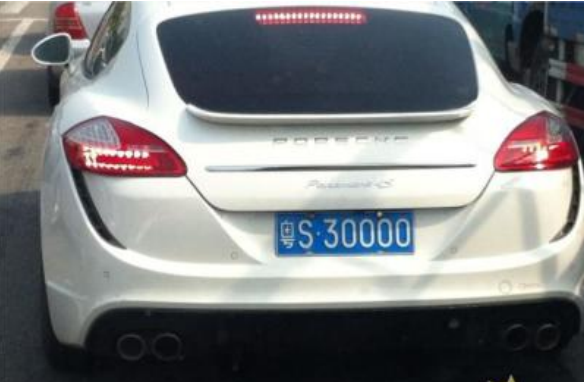
\includegraphics[scale=0.5]{figures/1.png}
	\caption{PageRank算法抽象图}
	\label{fig:1}
\end{figure}

\section{算法实现的流程与描述}
\begin{enumerate}[(1)]
	\item 从爬取所得到的数据集之中读取社交网络中各用户数据,并对各用户的PR值进行初始化设置,同时设置误差允许的范围p
	\item 根据用户之间的关系,利用PageRank算法对各用户之间的关系以及影响力进行计算。并且将用户自身的影响力有效分配给关注的用户。
	\item 再次对用户的影响力进行计算,直到与上轮误差达到预先设置的p值之内。这时可以认为读出来数据是准确的,并可以将其存入数据库以便进行下一步的继续研究。
\end{enumerate}

\section{基于图聚类的用户影响力算法}
\subsection{基于图聚类的算法}
图聚类算法原始是从聚类算法中延伸出来的,其中的数据对象通过结点来表示,并且用对应结点之间边的权值表示两个数据对象之间的邻近度。图聚类算法兼顾了聚类算法的核心思想并且利用了图的许多重要特性以及性质。下面是一些图聚类所用的重要方法。

\begin{enumerate}[(1)]
	\item 稀疏化邻近度图,只保留对象与其最向临近对象的链接。这种的稀疏化主要用于处理噪声和离群点。并且通过稀疏化也可以使得对稀疏图进行有效图划分算法。
	\item 基于共享的最近临个数。定义两个对象间的相似性的度量。这种方法主要用于在克服高维和变密度簇方面。
	\item 定义核心对象并构建环绕其间的簇。通过引进邻近度图或者稀疏化的邻近图的基于密度的分析,围绕核心对象并构建簇将会进一步发现不同形状和大小的簇。
	\item 使用邻近度图中所显示的信息,从而对两个簇是否应当合并作出更复杂的评估。
\end{enumerate}

\subsection{基于图聚类的社交网络聚类算法思想}
微博属于一种新兴的社交网络,拥有着成簇特性。本实验采用了社团发现算法,该算法类似于群的概念,团簇内部用户通过爱好,实际中的社交关系等联系在一起。且团簇彼此之间受影响较小。因此可以将各个团簇从微博网络中独立出来进行研究,对其利用复杂网络的聚类算法对社交网络用户进行聚类,分解出其团聚结构。
\par
本次实验所用的是一种改进的进行了平衡聚类事件和聚类精度的GN算法对社交网络用户行为进行聚类。该改进算法中将链接聚类系数定义为包含该路径的所有短回路数,计算i结点到j结点边的连接聚类系数公式如式3.2:
\begin{equation}
C_{i,j}^{g}=\frac{Z_{i,j}^{g}+1}{S_{i,j}^g}
\end{equation}
并且通过模块度函数用于评价网络聚类的终止条件,式3.3:
\begin{equation}
Q=\sum_{i}{(e_{ii}-a_i^2)}=Tre-\sum_{i}a_i^2
\end{equation}

本文使用的是Radicchi所提出的通过改进后的GN 算法对社交网络进行聚类,并且使用模块度函数作为聚类终止的判断条件。其算法流程如下:
\begin{enumerate}[(1)]
	\item 首先通过微博关注者与被关注者之间关系构建微博网络
	\item 计算Q值并通过判断是否终止聚类来进行划分
	\item 计算网络中所有连接边的连接聚类系数
	\item 删除连接聚类中系数最小的边
	\item 重复步骤(2)
\end{enumerate}
在对所搜集到的万级数据中对数据进行聚类,对Q取值为0.6。其所聚类迭代的次数以及所获得的团簇个数如表3.1所示。

\begin{table}[htbp]
	\centering
	\caption[迭代次数与团簇个数]{迭代次数与团簇个数}
	\begin{tabular}{|c|c|}
		\hline
		迭代次数 & 团簇个数\\
		\hline
		0 & 1\\
		\hline
		2&32\\
		\hline
		4&471\\
		\hline
		6&724\\
		\hline
		8&1534\\
		\hline
	\end{tabular}
\end{table}
从团簇的个数变化中可以看出,前6次的迭代中团簇分裂速度很快,第七次第八次分裂速度逐渐变慢最终分裂为1543个团簇。对其变化速率进行分析,发现其原因是在第七次迭代开始,社交网络中已经出现了大量满足Q值的团簇停止了其分裂过程。
团簇内部节点个数分布情况如表3.2所示

\begin{table}[htbp]
	\centering
	\caption[团簇内部结点个数]{团簇内部结点个数}
	\begin{tabular}{|c|c|}
		\hline
		簇内结点数 & 簇数\\
		\hline
		100及以下 & 1382\\
		\hline
		100-200&102\\
		\hline
		200-300&33\\
		\hline
		300-400&6\\
		\hline
		400以上&1\\
		\hline
	\end{tabular}
\end{table}
其中大部分的团簇中所包含的微博用户都少于100个,并且随着结点数的增加,所符合的团簇数目逐渐变小。团簇中最大结点数为478,最小值为1.其中90\%的团簇结点数少于100个。

\section{ 基于用户的微博团簇影响力计算}
本实验中主要所采取进行横向对比的是聚类的度中心度分布,介数中心度分布,距离中心度分布,距离中心度分布以及通过pagerank算法进行计算得出的网络用户影响力分析。
\begin{enumerate}[(1)]
	\item 粉丝数量:用户偏好在此次中即为用户对其他微博用户的关注度,对微博内容信息的转发评论等表示偏好的行为,当一个用户的粉丝数目越多时,其所发布的微博内容将会对更多的用户者偏好产生影响。因此大部分微博用户影响力评价模型中也将此作为一个计算因子。
	\item 微博数量:在社交网络中,用户发布微博是产生自身印象力并能对其他用户偏好产生影响的最好办法。微博的发布可以作为用户偏好以及影响力的传播载体,并且也可以体现用户在社交网络中的活跃程度。因此也将微博数量作为影响力计算因子。
\end{enumerate}
本实验中主要所采取进行横向对比的是聚类的度中心度分布,介数中心度分布,距离中心度分布,距离中心度分布以及通过pagerank算法进行计算得出的网络用户影响力分析。
下面用图3.2表示说明节点的各个性能:

\begin{figure}[h]
	\centering
	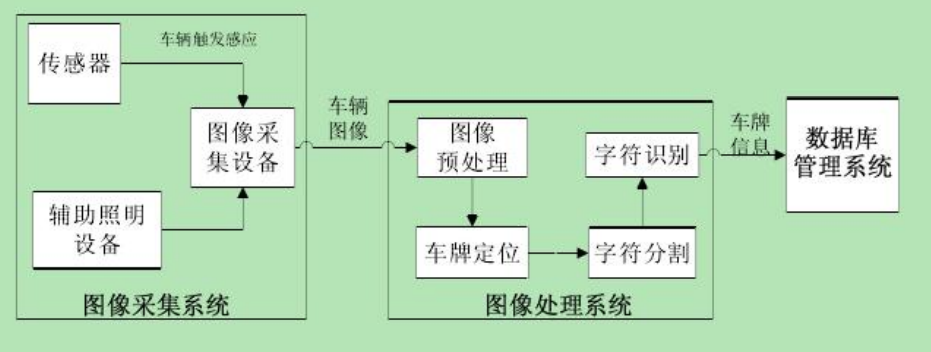
\includegraphics[scale=0.5]{figures/2.png}
	\caption{中心度的不同表示观点}
	\label{fig:1}
\end{figure}
\begin{enumerate}[(1)]
	\item 度中心度:是在网络分析之中刻画节点中心性的一个直接度量指标,一个节点的度中心度越大,则其中心性越高,在社交网络中所处的地位也就越重要。
	\item 距离中心度:决定了一个节点的紧密性。即该节点到达其他节点的难易程度。该性质是基于某一节点与社交网络中所有其他节点之间的平均最短路径长度计算而得到的。
	\item 介数中心度:核心思想是两个非邻接成员间的相互作用依赖于社交网络中的其他成员,特别是依赖于两成员间路径上的成员,它们对两个非邻接成员之间起着某种控制或依赖关系。如果一个成员A位于其他成员的多条最短路径上,那么成员A的作用就比较大,也具有较大的介数中心性。其本质为网络中包含成员B的所有最短路径条数占所有最短路径条数的百分比。
	\begin{equation}
	C_B(i)=\frac{\sum_{j<k}g_{jk}(i)}{g_{jk}}/[\frac{(n-1)(n-2)}{2}]
	\end{equation}
	其中$g_{jk}$表示连接j-k的最短路径的条数,$g_{jk}(i)$表示位于最短路径的个数。
\end{enumerate}







% !Mode:: "TeX:UTF-8"
\chapter{实验结果}
\section{灰度化}
结果如图4.1
\begin{figure}[h]
	\centering
	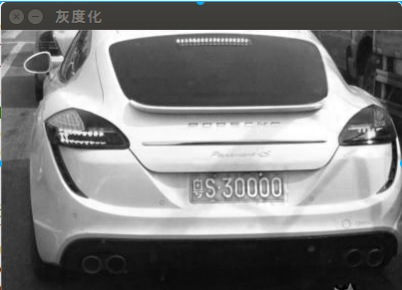
\includegraphics[scale=0.5]{figures/10.png}
	\caption{灰度化}
	\label{fig:2}
\end{figure}

\section{高斯滤波}
结果如图4.2
\begin{figure}[h]
	\centering
	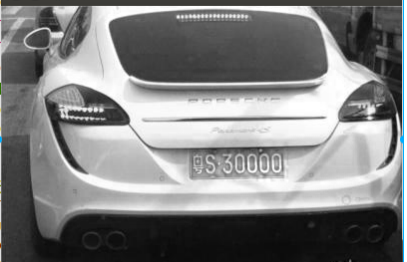
\includegraphics[scale=0.5]{figures/11.png}
	\caption{高斯滤波}
	\label{fig:2}
\end{figure}

\section{Sobol算子}
结果如图4.3
\begin{figure}[h]
	\centering
	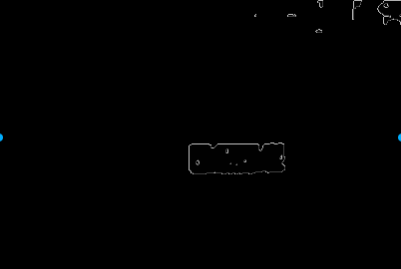
\includegraphics[scale=0.5]{figures/12.png}
	\caption{Sobol}
	\label{fig:2}
\end{figure}

\section{二值化}
结果如图4.4
\begin{figure}[h]
	\centering
	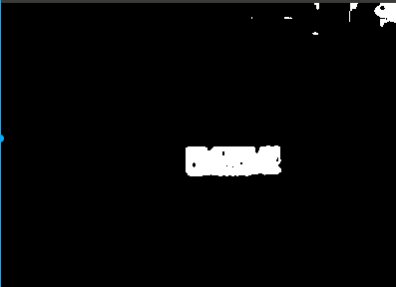
\includegraphics[scale=0.5]{figures/13.png}
	\caption{二值化}
	\label{fig:2}
\end{figure}

\section{闭运算}
结果如图4.5
\begin{figure}[h]
	\centering
	
\includegraphics[scale=0.5]{figures/14.png}
	\caption{闭运算}
	\label{fig:2}
\end{figure}

\section{定位}
\begin{enumerate}
	\item 简单车牌定位,结果如图4.6
	\item 复杂车牌定位,结果如图4.7
\end{enumerate}

\begin{figure}[h]
	\centering
	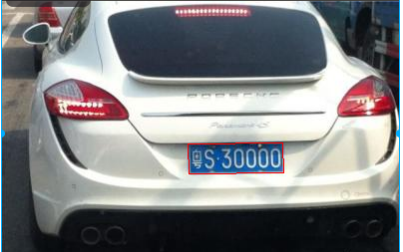
\includegraphics[scale=0.5]{figures/15.png}
	\caption{简单定位}
	\label{fig:2}
\end{figure}

\begin{figure}[h]
	\centering
	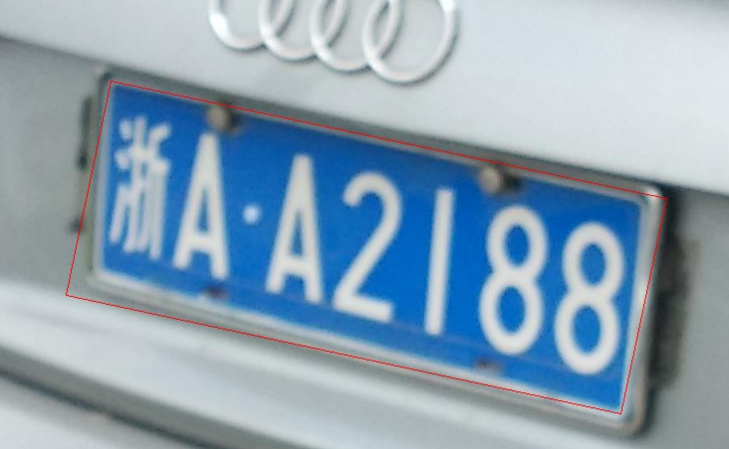
\includegraphics[scale=0.5]{figures/16.png}
	\caption{复杂定位}
	\label{fig:2}
\end{figure}

\section{字符分割}
结果如图4.8
\begin{figure}[h]
	\centering
	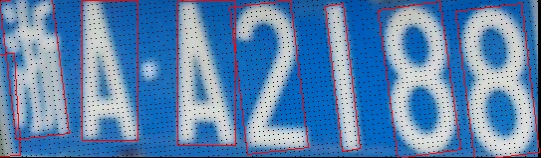
\includegraphics[scale=0.5]{figures/17.png}
	\caption{分割}
	\label{fig:2}
\end{figure}
\listoffigures                        % 插图索引
\listoftables                         % 表格索引
% 参考文献. 
\bibliographystyle{shuthesis}
\bibliography{reference/refs}

%\defaultfont
\BiAppendixChapter{������ʿѧλ�ڼ�������������}
{Papers Published in the Period of PH. D. Education}

\begin{publist}
\item ����. ��Ŀ. �ڿ�. ��, ��(��): ҳ��

\item ����. ��Ŀ. �ڿ�. ��, ��(��): ҳ��

\item ����. ��Ŀ. �ڿ�. ��, ��(��): ҳ��
\end{publist}
           % 发表论文清单
%% 致谢
\begin{acknowledgement}
  衷心感谢导师 xxx 教授对本人的精心指导. 
\end{acknowledgement}
        % 致谢

%\backmatter
%\begin{appendix}
%\chapter{经典不等式}
论文中用到的经典不等式.\\

\noindent{\bfseries (H\"older Inequality)}
设~$a_i\geq0$, $b_i\geq0$, $i=1$, $2$, $\cdots$, $n$, 且~$p>1$, $q>1$ 
满足~$1/p+1/q=1$. 则有
\[
\sum_{i=1}^{n}a_ib_i\leq\left(\sum_{i=1}^{n}a_i^p\right)^{\frac1p}
\cdot\left(\sum_{i=1}^{n}b_i^q\right)^{\frac1q},
\]
等号成立当且仅当存在一个常数~$c$ 满足~$a_i^p=cb_i^q$.\\

\noindent{\bfseries (PM Inequality)}
设~$x_1$, $x_2$, $\ldots$, $x_n$ 是~$n$ 个非负实数. 如果~$0<p<q$, 那么
\[
\left(\frac{x_1^p+x_2^p+\cdots+x_n^p}{n}\right)^{\frac{1}{p}}\leq
\left(\frac{x_1^q+x_2^q+\cdots+x_n^q}{n}\right)^{\frac{1}{q}},
\]
等号成立当且仅当~$x_1=x_2=\cdots =x_n$.\\

\noindent{\bfseries (AM-GM Inequality)}
设~$x_1$, $x_2$, $\ldots$, $x_n$ 是~$n$ 个非负实数. 则有
\[
\frac{x_1+x_2+\cdots+x_n}{n}\geq\sqrt[n]{x_1x_2\cdots x_n},
\]
等号成立当且仅当~$x_1=x_2=\cdots =x_n$.
%\end{appendix}

\end{document}
